% ============================================
% MODULAÇÃO ANGULAR: FM E PM
% ============================================

\subsection{Introdução}

\begin{frame}{Modulação Angular vs. Modulação em Amplitude}

\textbf{AM:} Amplitude varia, frequência e fase fixas
\[
s_{\AM}(t) = A(t) \cos(2\pi f_c t)
\]

\vspace{0.3cm}

\textbf{Modulação Angular:} Amplitude fixa, ângulo (fase ou frequência) varia
\[
s(t) = A_c \cos[\theta(t)] = A_c \cos[2\pi f_c t + \phi(t)]
\]

onde $\phi(t)$ é a fase modulada.

\vspace{0.5cm}

\textbf{Duas variantes:}

\begin{enumerate}
\item \textbf{FM (Modulação em Frequência):}
   
   Frequência instantânea varia com $m(t)$

\item \textbf{PM (Modulação em Fase):}
   
   Fase instantânea varia diretamente com $m(t)$
\end{enumerate}

\end{frame}

% ============================================

\begin{frame}{Fase e Frequência Instantâneas}

Para sinal modulado $s(t) = A_c \cos[\theta(t)]$:

\begin{block}{Definições}
\textbf{Fase instantânea:}
\[
\theta(t) = 2\pi f_c t + \phi(t)
\]

\textbf{Frequência instantânea:}
\[
f_i(t) = \frac{1}{2\pi} \frac{d\theta(t)}{dt} = f_c + \frac{1}{2\pi}\frac{d\phi(t)}{dt}
\]
\end{block}

\textbf{Interpretação:}
\begin{itemize}
\item $\theta(t)$: argumento da função cosseno
\item $f_i(t)$: taxa instantânea de oscilação
\item $f_c$: frequência da portadora (não modulada)
\item $\phi(t)$: desvio de fase causado pela modulação
\end{itemize}

\end{frame}

% ============================================

\subsection{Modulação em Frequência (FM)}

\begin{frame}{Definição de FM}

\begin{block}{Modulação em Frequência (FM)}
A frequência instantânea é proporcional à mensagem:
\[
f_i(t) = f_c + k_f m(t)
\]
onde $k_f$ é a constante de sensibilidade de frequência (Hz/V).
\end{block}

\textbf{Desvio de frequência:}
\[
\Delta f(t) = k_f m(t)
\]

\textbf{Desvio máximo:}
\[
\Delta f = k_f \max|m(t)|
\]

\vspace{0.3cm}

\textbf{Derivando} $\phi(t)$ de $f_i(t)$:

\[
\frac{d\phi(t)}{dt} = 2\pi k_f m(t) \quad \Rightarrow \quad \phi(t) = 2\pi k_f \int_{-\infty}^{t} m(\tau) d\tau
\]

\end{frame}

% ============================================

\begin{frame}{Sinal FM no Domínio do Tempo}

\begin{block}{Sinal FM}
\[
s_{\FM}(t) = A_c \cos\left[2\pi f_c t + 2\pi k_f \int_{-\infty}^{t} m(\tau) d\tau\right]
\]
\end{block}

Ou definindo o \textbf{índice de fase}:
\[
\beta(t) = 2\pi k_f \int_{-\infty}^{t} m(\tau) d\tau
\]

\[
s_{\FM}(t) = A_c \cos[2\pi f_c t + \beta(t)]
\]

\textbf{Características:}
\begin{itemize}
\item Amplitude constante: $|s_{\FM}(t)| = A_c$
\item Toda informação está na fase
\item Potência transmitida constante: $P_s = A_c^2/2$
\item \textbf{Vantagem:} Imune a variações de amplitude (ruído, desvanecimento)
\end{itemize}

\end{frame}

% ============================================

\begin{frame}{Modulação em Fase (PM)}

\begin{block}{Modulação em Fase (PM)}
A fase instantânea é diretamente proporcional à mensagem:
\[
\phi(t) = k_p m(t)
\]
onde $k_p$ é a constante de sensibilidade de fase (rad/V).
\end{block}

\textbf{Sinal PM:}
\[
s_{\PM}(t) = A_c \cos[2\pi f_c t + k_p m(t)]
\]

\textbf{Frequência instantânea:}
\[
f_i(t) = f_c + \frac{k_p}{2\pi} \frac{dm(t)}{dt}
\]

\textbf{Relação FM-PM:}
\begin{itemize}
\item \textbf{FM:} frequência $\propto m(t)$, fase $\propto \int m(t)dt$
\item \textbf{PM:} fase $\propto m(t)$, frequência $\propto dm(t)/dt$
\end{itemize}

\end{frame}

% ============================================

\begin{frame}{Relação entre FM e PM}

\textbf{FM pode ser vista como PM do integral:}

\[
\text{FM de } m(t) = \text{PM de } \int m(t)dt
\]

\textbf{PM pode ser vista como FM da derivada:}

\[
\text{PM de } m(t) = \text{FM de } \frac{dm(t)}{dt}
\]

\vspace{0.5cm}

\textbf{Conversão prática:}

\begin{center}
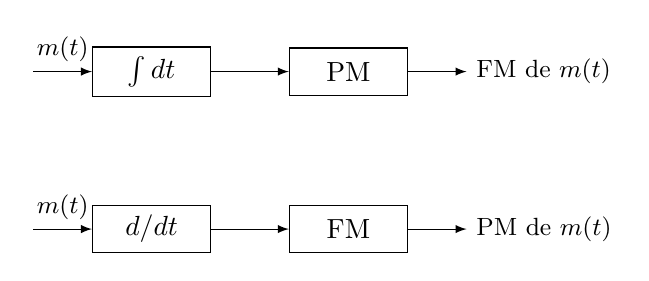
\begin{tikzpicture}[>=latex]
% FM para PM
\node[draw, rectangle, minimum width=1.5cm, minimum height=0.6cm] (int) at (0,1) {$\int dt$};
\node[draw, rectangle, minimum width=1.5cm, minimum height=0.6cm] (pm) at (2.5,1) {PM};
\draw[->] (-1.5,1) -- node[above, font=\small] {$m(t)$} (int);
\draw[->] (int) -- (pm);
\draw[->] (pm) -- (4,1) node[right, font=\small] {FM de $m(t)$};

% PM para FM
\node[draw, rectangle, minimum width=1.5cm, minimum height=0.6cm] (der) at (0,-1) {$d/dt$};
\node[draw, rectangle, minimum width=1.5cm, minimum height=0.6cm] (fm) at (2.5,-1) {FM};
\draw[->] (-1.5,-1) -- node[above, font=\small] {$m(t)$} (der);
\draw[->] (der) -- (fm);
\draw[->] (fm) -- (4,-1) node[right, font=\small] {PM de $m(t)$};
\end{tikzpicture}
\end{center}

\textbf{Na prática:} FM é mais comum (melhor desempenho em ruído)

\end{frame}

% ============================================

\subsection{Análise Espectral de FM}

\begin{frame}{FM com Tom Único: Configuração}

\textbf{Sinal modulante:} $m(t) = A_m \cos(2\pi f_m t)$

\textbf{Sinal FM:}
\[
s(t) = A_c \cos\left[2\pi f_c t + 2\pi k_f A_m \int_{-\infty}^{t} \cos(2\pi f_m \tau) d\tau\right]
\]

Integrando:
\[
\int \cos(2\pi f_m \tau) d\tau = \frac{\sin(2\pi f_m t)}{2\pi f_m}
\]

\[
s(t) = A_c \cos\left[2\pi f_c t + \frac{k_f A_m}{f_m} \sin(2\pi f_m t)\right]
\]

Definindo o \textbf{índice de modulação}:
\[
\beta = \frac{k_f A_m}{f_m} = \frac{\Delta f}{f_m}
\]

\[
\boxed{s(t) = A_c \cos[2\pi f_c t + \beta \sin(2\pi f_m t)]}
\]

\end{frame}

% ============================================

\begin{frame}{Expansão de Bessel}

\textbf{Para analisar o espectro, usamos a identidade:}

\[
\cos[\beta \sin(\omega_m t)] = \sum_{n=-\infty}^{\infty} J_n(\beta) \cos(n\omega_m t)
\]

onde $J_n(\beta)$ são \textbf{funções de Bessel de primeira espécie de ordem $n$}.

\vspace{0.3cm}

\textbf{Aplicando a} $s(t) = A_c \cos[2\pi f_c t + \beta \sin(2\pi f_m t)]$:

Usando $\cos(A + B) = \cos A \cos B - \sin A \sin B$:

\[
s(t) = A_c[\cos(2\pi f_c t)\cos(\beta \sin(2\pi f_m t)) - \sin(2\pi f_c t)\sin(\beta \sin(2\pi f_m t))]
\]

E as identidades:
\begin{align*}
\cos[\beta \sin(\omega_m t)] &= J_0(\beta) + 2\sum_{n=1}^{\infty} J_{2n}(\beta) \cos(2n\omega_m t) \\
\sin[\beta \sin(\omega_m t)] &= 2\sum_{n=0}^{\infty} J_{2n+1}(\beta) \sin[(2n+1)\omega_m t]
\end{align*}

\end{frame}

% ============================================

\begin{frame}{Espectro FM: Resultado Final}

Após manipulação algébrica:

\[
s(t) = A_c \sum_{n=-\infty}^{\infty} J_n(\beta) \cos[2\pi(f_c + nf_m)t]
\]

\textbf{Interpretação do espectro:}

\begin{itemize}
\item \textbf{Portadora} em $f_c$: amplitude $A_c J_0(\beta)$
\item \textbf{Bandas laterais} em $f_c \pm nf_m$ para $n = 1, 2, 3, ...$
\item Amplitude da n-ésima banda: $A_c J_n(\beta)$
\item \textbf{Infinitas bandas laterais teoricamente}
\item Na prática: $J_n(\beta) \approx 0$ para $n > \beta + 1$
\end{itemize}

\vspace{0.3cm}

\textbf{Diferença fundamental de AM:}
\begin{itemize}
\item AM: 2 bandas laterais (USB, LSB)
\item FM: Infinitas bandas laterais (mas só algumas significativas)
\end{itemize}

\end{frame}

% ============================================

\begin{frame}{Funções de Bessel}

\textbf{Propriedades importantes:}

\begin{itemize}
\item $J_{-n}(\beta) = (-1)^n J_n(\beta)$ (simetria)
\item $J_n(-\beta) = (-1)^n J_n(\beta)$
\item $\sum_{n=-\infty}^{\infty} J_n^2(\beta) = 1$ (conservação de potência!)
\item Para $\beta \ll 1$: $J_0(\beta) \approx 1$, $J_1(\beta) \approx \beta/2$, $J_n(\beta) \approx 0$ para $n \geq 2$
\end{itemize}

\vspace{0.3cm}

\textbf{Valores típicos:}

\begin{center}
\footnotesize
\begin{tabular}{|c|c|c|c|c|c|c|}
\hline
$\beta$ & $J_0$ & $J_1$ & $J_2$ & $J_3$ & $J_4$ & $J_5$ \\
\hline
0.5 & 0.94 & 0.24 & 0.03 & 0.00 & - & - \\
\hline
1.0 & 0.77 & 0.44 & 0.11 & 0.02 & 0.00 & - \\
\hline
2.0 & 0.22 & 0.58 & 0.35 & 0.13 & 0.03 & 0.01 \\
\hline
5.0 & -0.18 & -0.33 & 0.05 & 0.36 & 0.39 & 0.26 \\
\hline
\end{tabular}
\end{center}

\textbf{Veja figura:} Gráfico de $J_n(\beta)$ vs. $\beta$ para diferentes $n$

\end{frame}

% ============================================

\begin{frame}{Largura de Banda de FM}

\textbf{Problema:} Teoricamente, espectro FM tem largura infinita!

Na prática: Bandas com $|J_n(\beta)| < 0.01$ são desprezíveis.

\vspace{0.3cm}

\textbf{Número significativo de bandas laterais:}

Aproximadamente $n_{\max} \approx \beta + 1$

\textbf{Largura de banda aproximada:}
\[
B \approx 2n_{\max} f_m = 2(\beta + 1)f_m
\]

\begin{block}{Regra de Carson}
\[
\boxed{B_{\FM} \approx 2(\Delta f + f_m) = 2f_m(\beta + 1)}
\]
\end{block}

onde $\Delta f = k_f A_m$ é o desvio de frequência.

\textbf{Precisão:} Contém $\approx 98\%$ da potência do sinal FM.

\end{frame}

% ============================================

\begin{frame}{NBFM vs. WBFM}

\textbf{Dois regimes de operação:}

\begin{enumerate}
\item \textbf{NBFM (Narrowband FM):} $\beta \ll 1$
   \begin{itemize}
   \item $B \approx 2f_m$ (similar a AM)
   \item Poucas bandas laterais significativas
   \item Comportamento quase linear
   \end{itemize}

\item \textbf{WBFM (Wideband FM):} $\beta \gg 1$
   \begin{itemize}
   \item $B \approx 2\Delta f$ (dominado pelo desvio)
   \item Muitas bandas laterais
   \item Melhor desempenho em ruído
   \end{itemize}
\end{enumerate}

\vspace{0.3cm}

\textbf{Comparação com AM:}

\begin{itemize}
\item AM: $B = 2W$ (independente de $A_c$ ou $\mu$)
\item FM: $B = 2\Delta f(1 + 1/\beta)$ (depende de $\Delta f$!)
\item FM troca largura de banda por melhor SNR
\end{itemize}

\end{frame}

% ============================================

\begin{frame}{Exemplo 1: FM com Tom Único}

\textbf{Dados:}
\begin{itemize}
\item $m(t) = \cos(2\pi \times 5000 \cdot t)$ (5 kHz)
\item $\Delta f = 75$ kHz (desvio máximo)
\item $f_c = 100$ MHz (portadora)
\end{itemize}

\textbf{Cálculo do índice de modulação:}
\[
\beta = \frac{\Delta f}{f_m} = \frac{75 \text{ kHz}}{5 \text{ kHz}} = 15
\]

\textbf{Largura de banda (Carson):}
\[
B \approx 2(\Delta f + f_m) = 2(75 + 5) = 160 \text{ kHz}
\]

\textbf{Número de bandas significativas:}
\[
n_{\max} \approx \beta + 1 = 16
\]

$\rightarrow$ 16 pares de bandas laterais (32 componentes espectrais!)

\textbf{Classificação:} WBFM ($\beta = 15 \gg 1$)

\end{frame}

% ============================================

\begin{frame}{Exemplo 2: Rádio FM Comercial}

\textbf{Padrão FCC para FM broadcast:}

\begin{itemize}
\item Desvio máximo: $\Delta f = 75$ kHz
\item Frequência máxima de áudio: $f_m = 15$ kHz
\item Alocação de canal: 200 kHz
\end{itemize}

\textbf{Índice de modulação:}
\[
\beta = \frac{75 \text{ kHz}}{15 \text{ kHz}} = 5
\]

\textbf{Largura de banda necessária:}
\[
B = 2(\Delta f + f_m) = 2(75 + 15) = 180 \text{ kHz}
\]

\textbf{Observação:} Canal de 200 kHz acomoda 180 kHz + bandas de guarda

\vspace{0.3cm}

\textbf{Banda FM:} 88-108 MHz, espaçamento de 200 kHz

Número de canais: $(108-88)/0.2 = 100$ canais

\end{frame}

% ============================================

\subsection{Demodulação FM}

\begin{frame}{Princípios de Demodulação FM}

\textbf{Objetivo:} Recuperar $m(t)$ de $s_{\FM}(t) = A_c \cos[2\pi f_c t + 2\pi k_f \int m(\tau)d\tau]$

\vspace{0.3cm}

\textbf{Métodos principais:}

\begin{enumerate}
\item \textbf{Discriminador de frequência (slope detector)}
   \begin{itemize}
   \item Converte FM em AM, depois detecta envelope
   \end{itemize}

\item \textbf{Detector PLL (Phase-Locked Loop)}
   \begin{itemize}
   \item VCO "segue" a frequência de entrada
   \item Saída do VCO é proporcional a $m(t)$
   \end{itemize}

\item \textbf{Detector de Foster-Seeley}
   \begin{itemize}
   \item Usa transformador balanceado
   \end{itemize}

\item \textbf{Detector de razão (ratio detector)}
   \begin{itemize}
   \item Variante do Foster-Seeley
   \item Menos sensível a variações de amplitude
   \end{itemize}
\end{enumerate}

\end{frame}

% ============================================

\begin{frame}{Discriminador de Frequência}

\textbf{Princípio:} Converter variação de frequência em variação de amplitude

\begin{center}
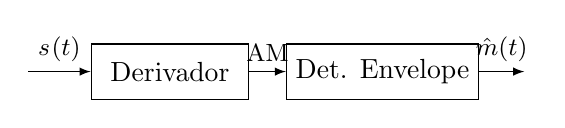
\begin{tikzpicture}[>=latex, scale=0.9]
\node[draw, rectangle, minimum width=2cm, minimum height=0.7cm] (der) at (0,0) {Derivador};
\node[draw, rectangle, minimum width=2cm, minimum height=0.7cm] (env) at (3,0) {Det. Envelope};

\draw[->] (-2,0) -- node[above, font=\small] {$s_{\FM}(t)$} (der);
\draw[->] (der) -- node[above, font=\small] {AM} (env);
\draw[->] (env) -- node[above, font=\small] {$\hat{m}(t)$} (5,0);
\end{tikzpicture}
\end{center}

\textbf{Análise matemática:}

\[
\frac{ds_{\FM}(t)}{dt} = -A_c \cdot 2\pi f_i(t) \sin[2\pi f_c t + \phi(t)]
\]

Amplitude do sinal derivado:
\[
A(t) = 2\pi A_c f_i(t) = 2\pi A_c [f_c + k_f m(t)]
\]

Após detector de envelope e filtro DC:
\[
\hat{m}(t) = K \cdot k_f m(t)
\]

\textbf{Problema:} Sensível a variações de amplitude (ruído AM)

\textbf{Solução:} Limitador de amplitude antes do discriminador

\end{frame}

% ============================================

\begin{frame}{Limitador de Amplitude}

\textbf{Propósito:} Remover variações de amplitude antes da demodulação FM

\begin{center}
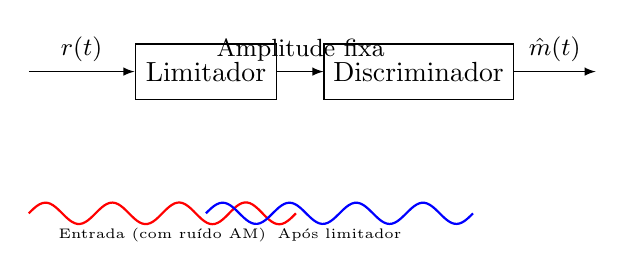
\begin{tikzpicture}[>=latex, scale=0.9]
\node[draw, rectangle, minimum width=1.8cm, minimum height=0.7cm] (lim) at (0,0) {Limitador};
\node[draw, rectangle, minimum width=2.2cm, minimum height=0.7cm] (disc) at (3,0) {Discriminador};

\draw[->] (-2.5,0) -- node[above, font=\small] {$r(t)$} (lim);
\draw[->] (lim) -- node[above, font=\small] {Amplitude fixa} (disc);
\draw[->] (disc) -- node[above, font=\small] {$\hat{m}(t)$} (5.5,0);

% Forma de onda de entrada (com variação de amplitude)
\begin{scope}[xshift=-2.5cm, yshift=-2cm, scale=0.15]
\draw[thick, red] plot[domain=0:8*pi, samples=100] (\x, {(1+0.3*sin(\x/4))*sin(\x r)});
\node[font=\tiny] at (4*pi,-2) {Entrada (com ruído AM)};
\end{scope}

% Forma de onda de saída (amplitude constante)
\begin{scope}[xshift=0cm, yshift=-2cm, scale=0.15]
\draw[thick, blue] plot[domain=0:8*pi, samples=100] (\x, {sin(\x r)});
\node[font=\tiny] at (4*pi,-2) {Após limitador};
\end{scope}
\end{tikzpicture}
\end{center}

\textbf{Implementação:}
\begin{itemize}
\item Amplificador com saturação (clipper)
\item Mantém informação de FM
\item Remove variações de amplitude
\end{itemize}

\textbf{Vantagem de FM:} Informação na frequência, não na amplitude!

\end{frame}

% ============================================

\subsection{PLL (Phase-Locked Loop)}

\begin{frame}{Conceito do PLL}

\textbf{PLL (Phase-Locked Loop):} Sistema de controle realimentado que sincroniza um oscilador local com sinal de entrada.

\begin{center}
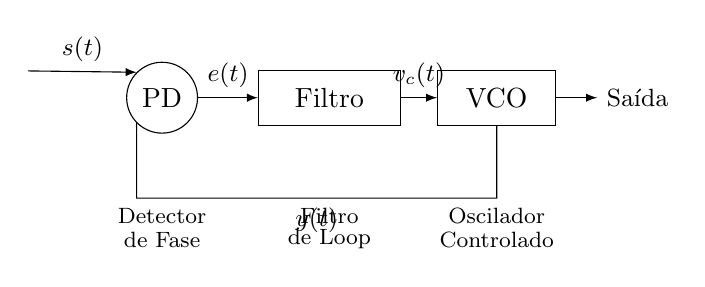
\begin{tikzpicture}[>=latex, scale=0.85]
% Detector de fase
\node[draw, circle, minimum size=0.9cm] (pd) at (0,0) {PD};
% Filtro
\node[draw, rectangle, minimum width=1.8cm, minimum height=0.7cm] (lpf) at (2.5,0) {Filtro};
% VCO
\node[draw, rectangle, minimum width=1.5cm, minimum height=0.7cm] (vco) at (5,0) {VCO};

% Conexões
\draw[->] (-2,0.4) -- node[above, font=\small] {$s(t)$} (pd.north west);
\draw[->] (pd.east) -- node[above, font=\small] {$e(t)$} (lpf.west);
\draw[->] (lpf.east) -- node[above, font=\small] {$v_c(t)$} (vco.west);
\draw[->] (vco.east) -- (6.5,0) node[right, font=\small] {Saída};

% Realimentação
\draw (vco.south) -- (5,-1.5) -| node[below, pos=0.25, font=\small] {$y(t)$} (pd.south west);

% Labels
\node[below of=pd, node distance=1.5cm, font=\footnotesize] {Detector};
\node[below of=pd, node distance=1.8cm, font=\footnotesize] {de Fase};
\node[below of=lpf, node distance=1.5cm, font=\footnotesize] {Filtro};
\node[below of=lpf, node distance=1.8cm, font=\footnotesize] {de Loop};
\node[below of=vco, node distance=1.5cm, font=\footnotesize] {Oscilador};
\node[below of=vco, node distance=1.8cm, font=\footnotesize] {Controlado};
\end{tikzpicture}
\end{center}

\textbf{Componentes:}
\begin{itemize}
\item \textbf{Detector de fase (PD):} Compara fases de entrada e VCO
\item \textbf{Filtro de loop:} Passa-baixas, define dinâmica
\item \textbf{VCO:} Frequência controlada por tensão
\end{itemize}

\end{frame}

% ============================================

\begin{frame}{Análise do PLL}

\textbf{Sinal de entrada FM:}
\[
s(t) = A_c \cos[2\pi f_c t + \phi_i(t)]
\]

\textbf{Saída do VCO:}
\[
y(t) = A_v \cos[2\pi f_c t + \phi_o(t)]
\]

\textbf{Detector de fase (multiplicador):}
\[
e(t) = K_d \sin[\phi_i(t) - \phi_o(t)] \approx K_d[\phi_i(t) - \phi_o(t)]
\]

para pequenos erros de fase.

\textbf{VCO:}
\[
\frac{d\phi_o(t)}{dt} = 2\pi K_v v_c(t)
\]

onde $K_v$ é a sensibilidade do VCO (Hz/V).

\end{frame}

% ============================================

\begin{frame}{Equação Diferencial do PLL}

\textbf{Filtro de loop:} $V_c(s) = F(s) E(s)$

\textbf{Análise em regime travado (locked):}

\[
\phi_o(t) \approx \phi_i(t)
\]

Para FM: $\phi_i(t) = 2\pi k_f \int m(\tau)d\tau$

VCO produz: $\frac{d\phi_o}{dt} = 2\pi K_v v_c(t)$

Igualando:
\[
v_c(t) = \frac{k_f}{K_v} m(t)
\]

\textbf{Conclusão:} $v_c(t)$ é proporcional a $m(t)$ $\rightarrow$ demodulação FM!

\begin{block}{Saída do PLL para FM}
\[
\boxed{v_c(t) = K m(t)}
\]
onde $K = k_f/K_v$ é o ganho de demodulação.
\end{block}

\end{frame}

% ============================================

\begin{frame}{Função de Transferência do PLL}

\textbf{No domínio de Laplace:}

Erro de fase: $E(s) = K_d[\Phi_i(s) - \Phi_o(s)]$

Filtro: $V_c(s) = F(s) E(s)$

VCO: $\Phi_o(s) = \frac{2\pi K_v}{s} V_c(s)$

\vspace{0.3cm}

\textbf{Função de transferência em malha fechada:}

\[
H(s) = \frac{\Phi_o(s)}{\Phi_i(s)} = \frac{K_d K_v F(s)}{s + K_d K_v F(s)}
\]

\textbf{Para filtro simples} $F(s) = 1$ (proporcional):

\[
H(s) = \frac{K_d K_v}{s + K_d K_v}
\]

Sistema de 1ª ordem com constante de tempo $\tau = 1/(K_d K_v)$

\textbf{Para filtro lag-lead:} Sistema de 2ª ordem (mais comum)

\end{frame}

% ============================================

\begin{frame}{Parâmetros do PLL}

\textbf{Largura de banda de captura (capture range):}

Faixa de frequências onde o PLL pode adquirir lock.

\[
\Delta f_{capture} \approx \frac{1}{2\pi} \sqrt{2 K_d K_v F(0)}
\]

\textbf{Largura de banda de lock (lock range):}

Faixa onde o PLL mantém lock após adquirido.

\[
\Delta f_{lock} \approx \frac{K_d K_v}{2\pi}
\]

Sempre: $\Delta f_{lock} > \Delta f_{capture}$

\vspace{0.3cm}

\textbf{Largura de banda de loop:}

Determina resposta dinâmica e rejeição de ruído.

Para filtro de 1ª ordem: $B_L = K_d K_v / (4\pi)$

\textbf{Trade-off:} Banda larga $\rightarrow$ resposta rápida, mas mais ruído

\end{frame}

% ============================================

\begin{frame}{Aplicações do PLL}

\textbf{O PLL é versátil e amplamente usado:}

\begin{enumerate}
\item \textbf{Demodulação FM:}
   \begin{itemize}
   \item Receptores FM de rádio e TV
   \item Excelente linearidade e rejeição de amplitude
   \end{itemize}

\item \textbf{Síntese de frequência:}
   \begin{itemize}
   \item Gerar múltiplos de frequência de referência
   \item Usado em geradores de RF
   \end{itemize}

\item \textbf{Recuperação de portadora:}
   \begin{itemize}
   \item Sistemas de comunicação digital
   \item Demodulação coerente
   \end{itemize}

\item \textbf{Recuperação de clock:}
   \begin{itemize}
   \item Sincronização de dados
   \item Interfaces seriais
   \end{itemize}

\item \textbf{Controle de motor:}
   \begin{itemize}
   \item Controle de velocidade preciso
   \end{itemize}
\end{enumerate}

\end{frame}

% ============================================

\subsection{Geração de FM}

\begin{frame}{Geração Direta de FM}

\textbf{Método: Modulador Direto com VCO}

\begin{center}
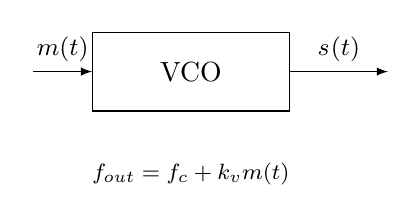
\begin{tikzpicture}[>=latex]
\node[draw, rectangle, minimum width=2.5cm, minimum height=1cm] (vco) at (0,0) {VCO};
\draw[->] (-2,0) -- node[above, font=\small] {$m(t)$} (vco.west);
\draw[->] (vco.east) -- node[above, font=\small] {$s_{\FM}(t)$} (2.5,0);
\node[below of=vco, node distance=1.3cm, font=\footnotesize] {$f_{out} = f_c + k_v m(t)$};
\end{tikzpicture}
\end{center}

\textbf{Características:}
\begin{itemize}
\item Simples e direto
\item $f_{out} = f_c + k_v m(t)$
\item VCO implementado com: varactor diode, capacitor variável, etc.
\end{itemize}

\textbf{Problema:} Instabilidade de frequência

\begin{itemize}
\item $f_c$ pode derivar com temperatura, componentes
\item Difícil obter $f_c$ precisa e estável
\end{itemize}

\textbf{Solução:} Usar método indireto (Armstrong)

\end{frame}

% ============================================

\begin{frame}{Método de Armstrong (Indireto)}

\textbf{Ideia:} Gerar NBFM estável, depois converter para WBFM

\textbf{Processo:}

\begin{enumerate}
\item Gerar NBFM com $\beta$ pequeno e $f_c$ estável (cristal)
\item Multiplicar frequência por $n$:
   \begin{itemize}
   \item $f_c \to nf_c$
   \item $\beta \to n\beta$
   \item $\Delta f \to n\Delta f$
   \end{itemize}
\item Converter para banda desejada (mixing)
\item Repetir multiplicação se necessário
\end{enumerate}

\vspace{0.3cm}

\textbf{Exemplo:}

Gerar FM com $f_c = 100$ MHz, $\Delta f = 75$ kHz:

\begin{itemize}
\item NBFM: $f_1 = 200$ kHz, $\Delta f_1 = 25$ Hz
\item Multiplicar por $\times 64$: $f_2 = 12.8$ MHz, $\Delta f_2 = 1.6$ kHz
\item Multiplicar por $\times 48$: $f_3 = 614.4$ MHz, $\Delta f_3 = 76.8$ kHz
\item Misturar com 514.4 MHz: $f_c = 100$ MHz, $\Delta f = 76.8$ kHz $\approx 75$ kHz
\end{itemize}

\end{frame}

% ============================================

\subsection{Receptor Superheterodino}

\begin{frame}{Princípio do Receptor Superheterodino}

\textbf{Problema:} Demodular diretamente em $f_c$ variável é complexo

\textbf{Solução:} Converter todas as frequências recebidas para uma \textbf{frequência intermediária (IF)} fixa

\begin{center}
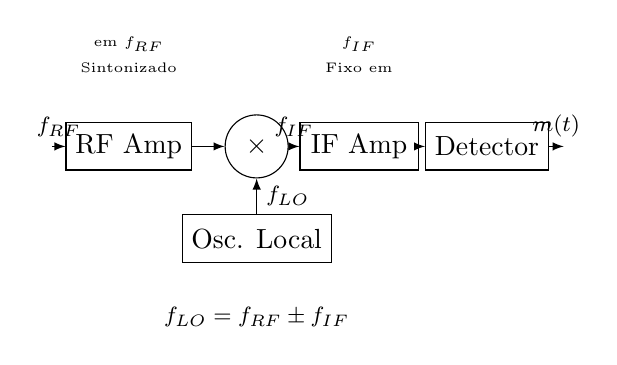
\begin{tikzpicture}[>=latex, scale=0.65]
% Blocos
\node[draw, rectangle, minimum width=1.5cm, minimum height=0.6cm] (rf) at (0,0) {RF Amp};
\node[draw, circle, minimum size=0.8cm] (mix) at (2.5,0) {$\times$};
\node[draw, rectangle, minimum width=1.5cm, minimum height=0.6cm] (if) at (4.5,0) {IF Amp};
\node[draw, rectangle, minimum width=1.5cm, minimum height=0.6cm] (det) at (7,0) {Detector};

% Oscilador local
\node[draw, rectangle, minimum width=1.5cm, minimum height=0.6cm] (lo) at (2.5,-1.8) {Osc. Local};

% Conexões
\draw[->] (-1.5,0) -- node[above, font=\footnotesize] {$f_{RF}$} (rf);
\draw[->] (rf) -- (mix.west);
\draw[->] (mix.east) -- node[above, font=\footnotesize] {$f_{IF}$} (if);
\draw[->] (if) -- (det);
\draw[->] (det) -- node[above, font=\footnotesize] {$m(t)$} (8.5,0);
\draw[->] (lo.north) -- node[right, font=\footnotesize] {$f_{LO}$} (mix.south);

% Labels
\node[above of=rf, node distance=1cm, font=\tiny] {Sintonizado};
\node[above of=rf, node distance=1.3cm, font=\tiny] {em $f_{RF}$};
\node[above of=if, node distance=1cm, font=\tiny] {Fixo em};
\node[above of=if, node distance=1.3cm, font=\tiny] {$f_{IF}$};
\node[below of=lo, node distance=1cm, font=\footnotesize] {$f_{LO} = f_{RF} \pm f_{IF}$};
\end{tikzpicture}
\end{center}

\textbf{Relação:}
\[
f_{IF} = |f_{RF} - f_{LO}|
\]

Ajustando $f_{LO}$, qualquer $f_{RF}$ é convertido para $f_{IF}$ fixo.

\end{frame}

% ============================================

\begin{frame}{Vantagens do Superheterodino}

\textbf{Vantagens:}

\begin{enumerate}
\item \textbf{Seletividade:}
   \begin{itemize}
   \item Filtro IF fixo pode ser muito seletivo
   \item Não precisa ajustar filtro ao trocar estação
   \end{itemize}

\item \textbf{Sensibilidade:}
   \begin{itemize}
   \item Amplificação concentrada em frequência fixa
   \item Melhor controle de ganho (AGC)
   \end{itemize}

\item \textbf{Estabilidade:}
   \begin{itemize}
   \item Osciladores em frequência fixa são mais estáveis
   \end{itemize}
\end{enumerate}

\textbf{Problema: Frequência Imagem}

Duas frequências produzem mesmo $f_{IF}$:
\begin{itemize}
\item Desejada: $f_s = f_{LO} + f_{IF}$
\item Imagem: $f_{im} = f_{LO} - f_{IF}$
\end{itemize}

\textbf{Solução:} Filtro de RF rejeita frequência imagem antes do mixer

\end{frame}

% ============================================

\begin{frame}{Exemplo: Receptor FM Superheterodino}

\textbf{Rádio FM comercial:}

\begin{itemize}
\item Banda FM: 88-108 MHz
\item IF padrão: $f_{IF} = 10.7$ MHz
\end{itemize}

\textbf{Para receber} $f_{RF} = 100.0$ MHz:

\[
f_{LO} = f_{RF} + f_{IF} = 100.0 + 10.7 = 110.7 \text{ MHz}
\]

\textbf{Frequência imagem:}
\[
f_{im} = f_{LO} + f_{IF} = 110.7 + 10.7 = 121.4 \text{ MHz}
\]

Fora da banda FM (88-108 MHz) $\rightarrow$ filtro RF facilmente rejeita

\vspace{0.3cm}

\textbf{Processamento:}
\begin{itemize}
\item Amplificador RF sintonizado em 100 MHz
\item Mixer com LO de 110.7 MHz
\item Amplificador IF em 10.7 MHz (filtro muito seletivo)
\item Discriminador FM ou PLL para demodular
\end{itemize}

\end{frame}

% ============================================

\subsection{FDM}

\begin{frame}{Multiplexação por Divisão de Frequência}

\textbf{FDM (Frequency Division Multiplexing):}

Múltiplos sinais compartilham mesmo canal, cada um em frequência diferente.

\begin{center}
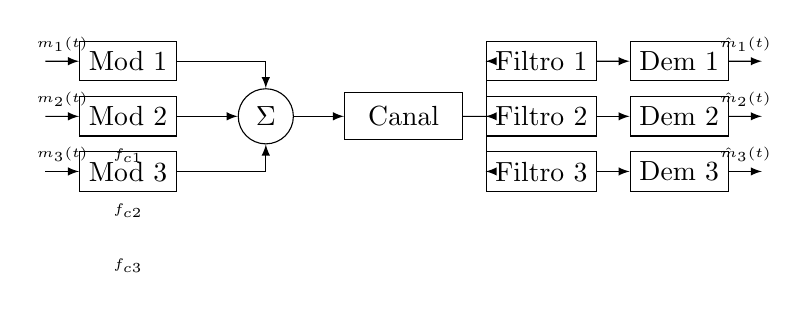
\begin{tikzpicture}[>=latex, scale=0.7]
% Transmissor
\node[draw, rectangle, minimum width=1.2cm, minimum height=0.5cm] (m1) at (0,2) {Mod 1};
\node[draw, rectangle, minimum width=1.2cm, minimum height=0.5cm] (m2) at (0,1) {Mod 2};
\node[draw, rectangle, minimum width=1.2cm, minimum height=0.5cm] (m3) at (0,0) {Mod 3};
\node[draw, circle, minimum size=0.7cm] (sum) at (2.5,1) {$\Sigma$};
\node[draw, rectangle, minimum width=1.5cm, minimum height=0.6cm] (canal) at (5,1) {Canal};

% Receptor
\node[draw, rectangle, minimum width=1.2cm, minimum height=0.5cm] (f1) at (7.5,2) {Filtro 1};
\node[draw, rectangle, minimum width=1.2cm, minimum height=0.5cm] (f2) at (7.5,1) {Filtro 2};
\node[draw, rectangle, minimum width=1.2cm, minimum height=0.5cm] (f3) at (7.5,0) {Filtro 3};
\node[draw, rectangle, minimum width=1.2cm, minimum height=0.5cm] (d1) at (10,2) {Dem 1};
\node[draw, rectangle, minimum width=1.2cm, minimum height=0.5cm] (d2) at (10,1) {Dem 2};
\node[draw, rectangle, minimum width=1.2cm, minimum height=0.5cm] (d3) at (10,0) {Dem 3};

% Conexões TX
\draw[->] (-1.5,2) -- node[above, font=\tiny] {$m_1(t)$} (m1);
\draw[->] (-1.5,1) -- node[above, font=\tiny] {$m_2(t)$} (m2);
\draw[->] (-1.5,0) -- node[above, font=\tiny] {$m_3(t)$} (m3);
\draw[->] (m1) -| (sum.north);
\draw[->] (m2) -- (sum.west);
\draw[->] (m3) -| (sum.south);
\draw[->] (sum) -- (canal);

% Conexões RX
\draw (canal.east) -- (6.5,1);
\draw[->] (6.5,1) |- (f1);
\draw[->] (6.5,1) -- (f2);
\draw[->] (6.5,1) |- (f3);
\draw[->] (f1) -- (d1);
\draw[->] (f2) -- (d2);
\draw[->] (f3) -- (d3);
\draw[->] (d1) -- node[above, font=\tiny] {$\hat{m}_1(t)$} (11.5,2);
\draw[->] (d2) -- node[above, font=\tiny] {$\hat{m}_2(t)$} (11.5,1);
\draw[->] (d3) -- node[above, font=\tiny] {$\hat{m}_3(t)$} (11.5,0);

% Portadoras
\node[below of=m1, node distance=1.2cm, font=\tiny] {$f_{c1}$};
\node[below of=m2, node distance=1.2cm, font=\tiny] {$f_{c2}$};
\node[below of=m3, node distance=1.2cm, font=\tiny] {$f_{c3}$};
\end{tikzpicture}
\end{center}

\textbf{Requisito:} $f_{ci}$ suficientemente espaçadas para evitar sobreposição espectral

\textbf{Aplicações:} TV a cabo, telefonia analógica (hierarquia FDM)

\end{frame}

% ============================================

\begin{frame}{Exemplo: FDM em Telefonia}

\textbf{Hierarquia FDM analógica (histórica):}

\begin{itemize}
\item \textbf{Grupo:} 12 canais de voz (4 kHz cada)
  \begin{itemize}
  \item SSB-LSB, espaçamento de 4 kHz
  \item Faixa: 60-108 kHz
  \item Banda total: 48 kHz
  \end{itemize}

\item \textbf{Supergrupo:} 5 grupos = 60 canais
  \begin{itemize}
  \item Faixa: 312-552 kHz
  \item Banda: 240 kHz
  \end{itemize}

\item \textbf{Grupo mestre:} 10 supergrupos = 600 canais
  \begin{itemize}
  \item Faixa: 564-3084 kHz
  \item Banda: 2520 kHz
  \end{itemize}
\end{itemize}

\vspace{0.3cm}

\textbf{Nota:} Substituído por sistemas digitais (TDM, SONET/SDH), mas princípio permanece em sistemas ópticos (WDM).

\end{frame}

% ============================================

\begin{frame}{Resumo: Modulação Angular}

\textbf{FM vs. PM:}
\begin{itemize}
\item FM: frequência $\propto m(t)$, fase $\propto \int m(t)$
\item PM: fase $\propto m(t)$, frequência $\propto dm(t)/dt$
\item FM mais comum (melhor em ruído)
\end{itemize}

\vspace{0.3cm}

\textbf{Espectro FM:}
\begin{itemize}
\item Infinitas bandas laterais (Bessel)
\item Largura de banda: $B \approx 2(\Delta f + f_m)$ (Carson)
\item NBFM: $\beta \ll 1$, WBFM: $\beta \gg 1$
\end{itemize}

\vspace{0.3cm}

\textbf{Demodulação:}
\begin{itemize}
\item Discriminador de frequência
\item PLL (mais usado atualmente)
\end{itemize}

\vspace{0.3cm}

\textbf{Geração:}
\begin{itemize}
\item Direta: VCO (instável)
\item Indireta: Armstrong (estável)
\end{itemize}

\end{frame}
